\section{Das Nautische Dreieck}
\subsection{Definition des Nautischen Dreiecks}
Ursprünglich ist das nautische Dreieck ein Hilfsmittel der sphärischen Astronomie um die momentane Position eines Fixsterns oder Planeten an der Himmelskugel. 
Die Himmelskugel ist eine gedachte Kugel, welche die Erde und dessen Beobachter umgibt und als Rechenfläche für Koordinaten in der Astronomie und Geodäsie dient.
Das nautische Dreieck definiert sich durch folgende Ecken: Zenit, Gestirn und Himmelspol.

Der Zenit ist jener Punkt, der vom Erdmittelpunkt durch denn eigenen Standort an die Himmelskugel verlängert wird.
Ein Gestirn ist ein Planet oder ein Fixstern, zu welchen es diverse Jahrbücher mit allen astronomischen Eigenschaften gibt. 
Der Himmelspol ist der Nordpol an die Himmelskugel projiziert.

Zur Anwendung der Formeln der sphärischen Trigonometrie gelten folgende einfache Zusammenhänge:
\begin{itemize}
	\item Seitenlänge Zenit zu Himmelspol $= \frac{\pi}{2} - \phi $
	\item Seitenlänge Himmelspol zu Gestirn $= \frac{\pi}{2} - \delta$
	\item Seitenlänge Zenit zu Gestirn $= \frac{\pi}{2} - h$
	\item Winkel von Zenit zu Himmelsnordpol zu Gestirn$=\pi - \alpha$
	\item Winkel von Himmelsnordpol zu Zenit und Gestirn$= \tau$
\end{itemize}
Um mit diesen Zusammenhängen zu rechnen benötigt man folgende Legende:
\begin{center}
	\begin{tabular}{ c c c }
		Winkel && Name / Beziehung \\ 
		\hline
		$\alpha$ && Rektaszension \\  
		$\delta$ && Deklination \\
		$\theta$ && Sternzeit von Greenwich\\
		$\phi$  &&  Geographische Breite\\
		$\tau=\theta-\alpha$ && Stundenwinkel und Längengrad des Gestirns. \\
		$a$ &&      Azimut\\
		$h$ &&      Höhe
	\end{tabular}
\end{center}

\subsection{Zusammenhang des nautischen Dreiecks und des Kugeldreiecks auf der Erdkugel}
\begin{figure}
	\begin{center}
		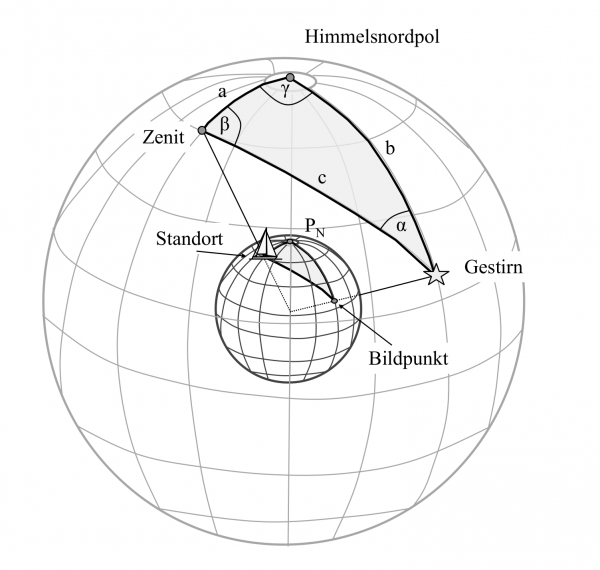
\includegraphics[height=5cm,width=8cm]{papers/nav/bilder/kugel3.png}
		\caption[Nautisches Dreieck]{Nautisches Dreieck}
	\end{center}
\end{figure}

Wie man im oberen Bild sieht, liegt das nautische Dreieck auf der Himmelskugel mit den Ecken Zenit, Gestirn und Himmelsnordpol. 
Das selbe Dreieck kann man aber auch auf die Erdkugel projizieren und es hat dann die Ecken Standort, Bildpunkt und Nordpol. 
Als Bildpunkt wird in der astronomischen Navigation der Punkt bezeichnet, an dem eine gedachte Linie vom Mittelpunkt eines beobachteten Gestirns zum Mittelpunkt der Erde die Erdoberfläche schneidet.


\section{Standortbestimmung ohne elektronische Hilfsmittel}
Um den eigenen Standort herauszufinden, wird in diesem Kapitel die Projektion Nautische Dreieck auf der Erdkugel zur Hilfe genommen. 
Mithilfe einiger Hilfsmittel und der Sphärischen Trigonometrie kann man dann die Längen- und Breitengrade des eigenen Standortes bestimmen.

\begin{figure}
	\begin{center}
		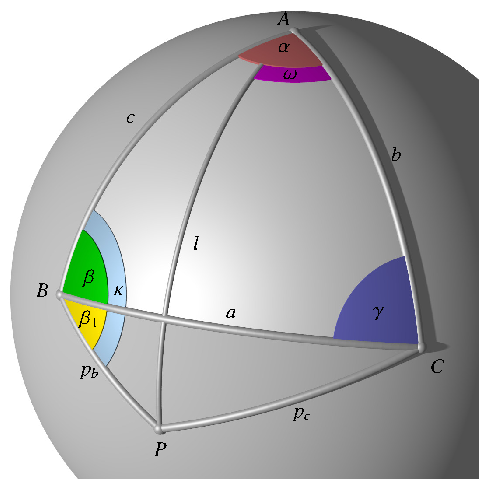
\includegraphics[width=10cm]{papers/nav/bilder/dreieck.pdf}
		\caption[Dreieck für die Standortbestimmung]{Dreieck für die Standortbestimmung}
	\end{center}
\end{figure}




\subsection{Ecke $P$ und $A$}
Unser eigener Standort ist der gesuchte Ecke $P$ und die Ecke $A$ ist in unserem Fall der Nordpol.
Der Vorteil ander Idee des Nautischen Dreiecks ist, dass eine Ecke immer der Nordpol ist. 
Somit ist diese Ecke immer bekannt und nur deswegen sind die Zusammenhänge von Rektaszension, Sternzeit und Deklination so simpel.

\subsection{Ecke $B$ und $C$ - Bildpunkt X und Y}
Für die Standortermittlung benötigt man als weiteren Punkt ein Gestirn bzw. seinen Bildpunkt auf der Erdkugel. 
Damit das trigonometrische Rechnen einfacher wird, werden hier zwei Gestirne zur Hilfe genommen.
Es gibt diverse Gestirne, die man nutzen kann wie zum Beispiel die Sonne, der Mond oder die vier Navigationsplaneten Venus, Mars, Jupiter und Saturn.

\subsection{Ephemeriden}
Zu all diesen Gestirnen gibt es Ephemeriden, die man auch Jahrbücher nennt. 
In diesen findet man Begriffe wie Rektaszension, Deklination und Sternzeit.
Da diese Angaben in Stundenabständen gegeben sind, muss man für die minutengenaue Bestimmung zwischen den Stunden interpolieren.
Was diese Begriffe bedeuten, wird in den kommenden beiden Abschnitten erklärt.

\begin{figure}
	\begin{center}
		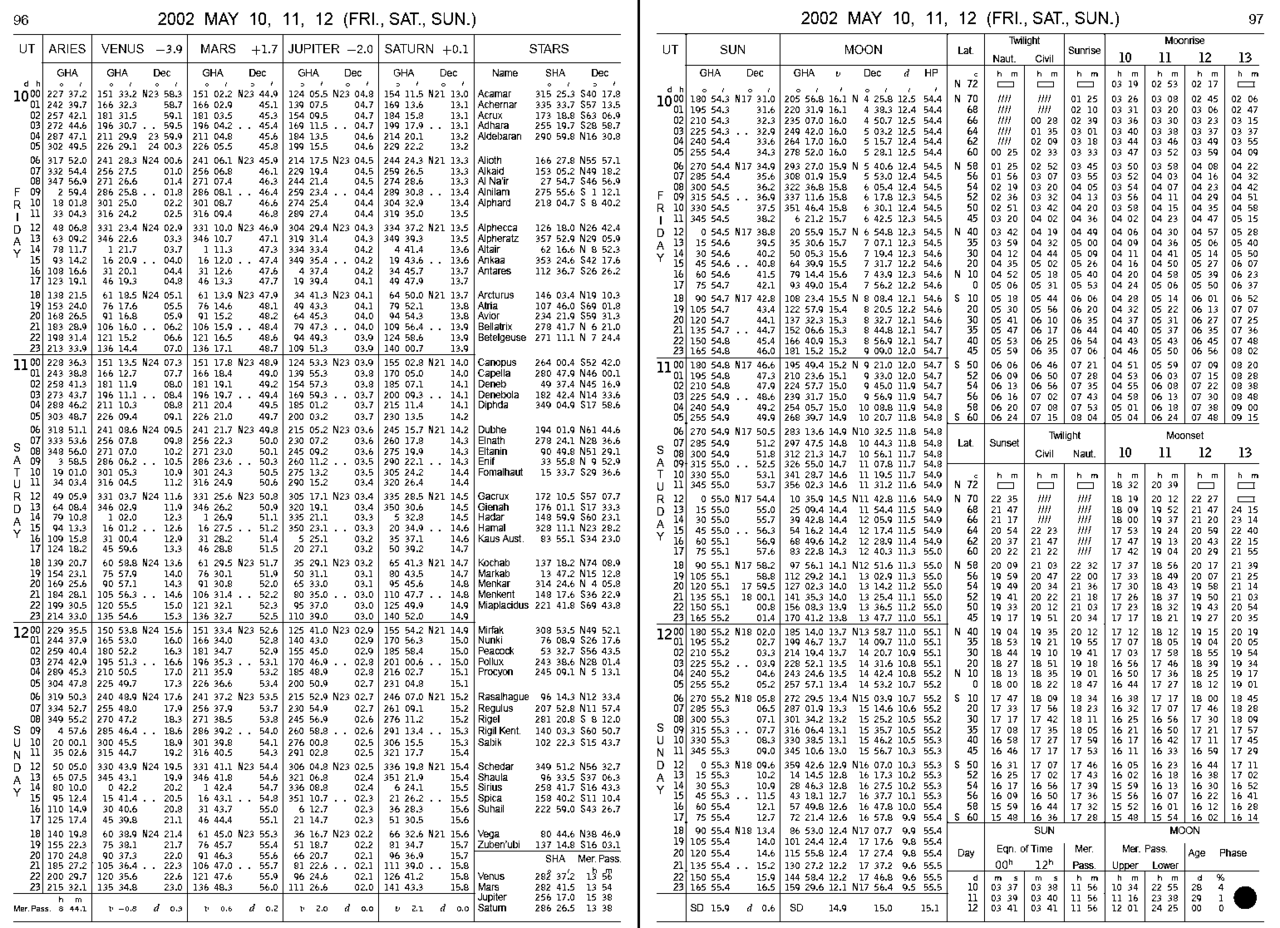
\includegraphics[width=18cm]{papers/nav/bilder/ephe.png}
		\caption[Astrodienst - Ephemeriden Januar 2022]{Astrodienst - Ephemeriden Januar 2022}
	\end{center}
\end{figure}

\subsubsection{Deklination}
Die Deklination $\delta$ beschreibt den Winkel zwischen dem Himmelsäquator und Gestirn und ergibt schlussendlich den Breitengrad.

\subsubsection{Sternzeit und Rektaszension}
Die Rektaszension $\alpha$ gibt an, in welchem Winkel das Gestirn zum Frühlingspunkt steht und geht vom Koordinatensystem der Himmelskugel aus.
Der Frühlungspunkt ist der Nullpunkt auf dem Himmelsäquator. 
Die Tatsache, dass sich die Himmelskugel  ca. vier Minuten schneller um die eigene Achse dreht als die Erdkugel, stellt hier ein kleines Problem dar.
Die Lösung ist die Sternzeit. 
Mit dieser können wir die schnellere Drehung der Himmelskugel ausgleichen und können die 
Am Frühlingspunkt (21. März) 12:00 Uhr ist die Sternzeit
$\theta = 0$. 

Die Sternzeit geht vom Frühlungspunkt aus, an welchem die Sonne den Himmelsäquator schneidet.
Für die Standortermittlung auf der Erdkugel ist es am einfachsten, wenn man die Sternzeit von Greenwich berechnet. 
Für die Sternzeit von Greenwich $\theta $braucht man als erstes das Julianische Datum $T$ vom aktuellen Tag, welches sich leicht recherchieren lässt.
Im Anschluss berechnet man die Sternzeit von Greenwich

$\theta = 6^h 41^m 50^s,54841 + 8640184^s,812866 \cdot T + 0^s,093104 \cdot T^2 - 0^s,0000062 \cdot T^3$.

Wenn mann die Sternzeit von Greenwich ausgerechnet hat, kann man den Längengrad des Gestirns $\lambda = \theta - \alpha$ mithilfe der Rektaszension und Sternzeit von Greenwich bestimmen. 
Dies gilt analog auch für das zweite Gestirn.

\subsection{Bestimmung des eigenen Standortes P}
Nun hat man die Koordinaten der beiden Gestirne und man weiss die Koordinaten des Nordpols.
Damit wir unseren Standort bestimmen können, bilden wir zuerst das Dreieck $ABC$, dann das Dreieck $BPC$ und zum Schluss noch das Dreieck $ABP$.
Mithilfe dieser Dreiecken können wir die einfachen Sätze der sphärischen Trigonometrie anwenden und benötigen lediglich ein Ephemeride zu den Gestirnen und einen Sextant.

\begin{figure}
	\begin{center}
		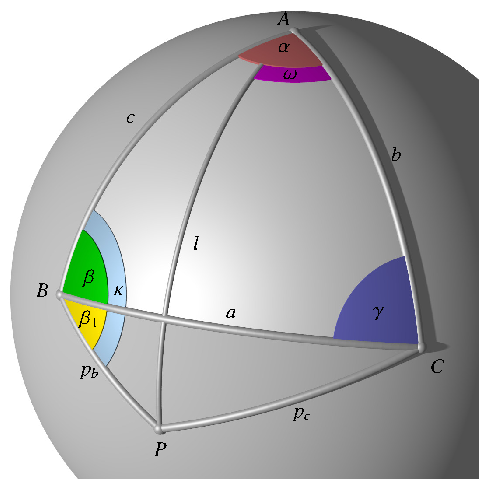
\includegraphics[width=10cm]{papers/nav/bilder/dreieck.pdf}
		\caption[Dreieck für die Standortbestimmung]{Dreieck für die Standortbestimmung}
	\end{center}
\end{figure}


\subsubsection{Dreieck $ABC$}

\begin{center}
	\begin{tabular}{ c c c }
		Ecke && Name  \\ 
		\hline
		$A$ && Nordpol \\  
		$B$ && Bildpunkt des Gestirns $X$ \\
		$C$&& Bildpunkt des Gestirns $Y$
	\end{tabular}
\end{center}

Mithilfe des sphärischen Trigonometrie und den darausfolgenden Zusammenhängen des Nautischen Dreiecks können wir nun alle Seiten des Dreiecks $ABC$ berechnen.

Die Seitenlänge der Seite "Nordpol zum Bildpunkt X" sei $c$. 
Dann ist $c = \frac{\pi}{2} - \delta_1$. 

Die Seitenlänge der Seite "Nordpol zum Bildpunkt Y" sei $b$.
Dann ist $b = \frac{\pi}{2} - \delta_2$. 

Der Innenwinkel beim der Ecke "Nordpol" sei $\alpha$.
Dann ist $ \alpha = |\lambda_1 - \lambda_2|$. 

mit 
\begin{center}
	\begin{tabular}{ c c c }
		Ecke && Name  \\ 
		\hline
		$\delta_1$ && Deklination Bildpunkt $X$ \\  
		$\delta_2$ && Deklination Bildpunk $Y$ \\
		$\lambda_1 $&& Längengrad Bildpunkt $X$\\
		$\lambda_2$ && Längengrad Bildpunkt $Y$
	\end{tabular}
\end{center}

Wichtig ist: Die Differenz der Längengrade ist gleich der Innenwinkel Alpha, deswegen der Betrag!

Nun haben wir die beiden Seiten $c\ und\ b$ und den Winkel $\alpha$, der sich zwischen diesen Seiten befindet. 
Mithilfe des Seiten-Kosinussatzes 
$\cos(a) = \cos(b)\cdot \cos(c) + \sin(b) \cdot \sin(c)\cdot \cos(\alpha)$ 
können wir nun die dritte Seitenlänge bestimmen. 
Es ist darauf zu achten, dass hier natürlich die Seitenlängen in Bogenmass sind und dementsprechend der Kosinus und Sinus verwendet wird. 

Jetzt fehlen noch die beiden anderen Innenwinkel $\beta \ und\ \gamma$.
Diese bestimmen wir mithilfe des Sinussatzes $\frac{\sin (a)}{\sin (\alpha)} =\frac{\sin (b)}{\sin (\beta)} = \frac{\sin (c)}{\sin (\gamma)}$.
Hier muss man aufpassen, dass man Seite von Winkel unterscheiden kann. 
Im Zähler sind die Seiten, im Nenner die Winkel. 
Somit ist $\beta =\sin^{-1} [\sin(b) \cdot \frac{\sin(\alpha)}{\sin(a)}] $.

Schlussendlich haben wir die Seiten $a,b\ und \ c$, die Ecken A,B und C und die Winkel $\alpha, \beta \ und \ \gamma$ bestimmt und somit das ganze erste Kugeldreieck berechnet.

\subsubsection{Dreieck $BPC$}
Wir bilden nun ein zweites Dreieck, welches die Ecken B und C des ersten Dreiecks besitzt. 
Die dritte Ecke ist der eigene Standort P.
Unser Standort definiere sich aus einer geographischen Breite $\delta$ und einer geographischen Länge $\lambda$. 

Die Seite von P zu B sei $pb$ und die Seite von P zu C sei $pc$.
Die beiden Seitenlängen kann man mit dem Sextant messen und durch eine einfache Formel bestimmen, nämlich $pb=\frac{\pi}{2} - h_{B}$ und $pc=\frac{\pi}{2} - h_{C}$ 

mit $h_B=$ Höhe von Gestirn in B und $h_C=$ Höhe von Gestirn in C mit Sextant gemessen.

Zum Schluss müssen wir noch den Winkel $\beta1$ mithilfe des Seiten-Kosinussatzes  mit den bekannten Seiten $pc$, $pb$ und $a$ bestimmen.
\subsubsection{Dreieck $ABP$}
Nun muss man eine Verbindungslinie ziehen zwischen P und A. Die Länge $l$ dieser Linie entspricht der gesuchten geographischen Breite $\delta$. Diese lässt sich mithilfe des Dreiecks $ABP$, den bekannten Seiten $c\ und \ pb$ und des Seiten-Kosinussatzes berechnen.

Für den Seiten-Kosinussatz benötigt es noch $\kappa=\beta + \beta1$.

Somit ist $\cos(l) = \cos(c)\cdot \cos(pb) + \sin(c) \cdot \sin(pb) \cdot \cos(\kappa)$

und

\[
\delta  =\cos^{-1} [\cos(c) \cdot \cos(pb) + \sin(c) \cdot \sin(pb) \cdot \cos(\kappa)].
\]

Für die Geographische Länge $\lambda$ des eigenen Standortes muss man den Winkel $\omega$, welcher sich im Dreieck $ACP$ in der Ecke bei $A$ befindet mithilfe des Sinussatzes $\frac{\sin (a)}{\sin (\alpha)} =\frac{\sin (b)}{\sin (\beta)} = \frac{\sin (c)}{\sin (\gamma)}$ bestimmen. 

Somit ist \[ \omega=\sin^{-1}[\sin(pc) \cdot \frac{\sin(\gamma)}{\sin(l)}] \]und unsere gesuchte geographische Länge schlussendlich 
\[\lambda=\lambda_1 - \omega\]
mit $\lambda_1$=Längengrad Bildpunkt $X
